% Dense validation companion manuscript scaffold.
%
% Compile from this directory:
%   latexmk -pdf dense_validation_report.tex
%
% This document is intended as a sister manuscript/report to
% DownscalingMoistureModel/paper/paper.pdf.  It deliberately treats model 6 and
% model 8 as already-defined models and focuses on dense, paddock-scale
% validation evidence.

\documentclass[11pt,a4paper]{article}

\usepackage[margin=2.5cm]{geometry}
\usepackage{graphicx}
\usepackage{booktabs}
\usepackage{amsmath}
\usepackage{microtype}
\usepackage{xcolor}
\usepackage{array}
\usepackage{tabularx}
\usepackage[round]{natbib}
\usepackage[hidelinks]{hyperref}

\graphicspath{
  {../unified_dense_validation/figures/}
  {../unified_dense_validation/figures/stage1/}
  {../unified_dense_validation/figures/stage1/dem_point_overlays/}
  {../unified_dense_validation/figures/stage1/quality_surfaces/}
  {../unified_dense_validation/figures/stage1/llara_native_prediction_maps/}
  {../unified_dense_validation/figures/stage2_local_spiking/}
}

\newcommand{\nse}{\ensuremath{\mathrm{NSE}}}
\newcommand{\ubrmse}{\ensuremath{\mathrm{ubRMSE}}}
\newcommand{\pearsonr}{\ensuremath{r}}
\newcommand{\vwc}{\ensuremath{\mathrm{VWC}}}
\newcommand{\modelSix}{model~6 RF}
\newcommand{\modelEight}{model~8 process}
\newcommand{\smips}{\texttt{SMIPS TotalBucket}}
\definecolor{cautioncolor}{RGB}{185,95,0}
\newcommand{\todo}[1]{\textcolor{red}{[TODO: #1]}}
\newcommand{\caution}[1]{\textcolor{cautioncolor}{[Caution: #1]}}
\newcommand{\placeholderbox}[2]{%
  \begin{center}
  \fbox{\begin{minipage}{0.92\linewidth}
  \vspace{0.7em}
  \textbf{#1}\par
  \vspace{0.35em}
  #2
  \vspace{0.7em}
  \end{minipage}}
  \end{center}
}

\title{Dense paddock-scale validation of statistical and process-based
soil-moisture downscaling}
\author{Dmitry [surname]\thanks{[affiliation; email]} \and
Yasar Adeel Ansari\thanks{[affiliation; email]}}
\date{Draft --- \today}

\begin{document}

\maketitle

\begin{center}
\begin{minipage}{0.9\textwidth}\small\itshape
Companion validation report to ``Downscaling SMIPS soil moisture to 30\,m:
statistical and process-based estimation of root-zone soil moisture, with
validation in the Murrumbidgee catchment''.  This draft scaffold separates the
model-development evidence from the dense-site validation evidence.  Red
\todo{items} should be resolved before circulation.
\end{minipage}
\end{center}

\begin{abstract}
\todo{Write after results are stabilised. Suggested structure: one sentence on
the paddock-scale validation gap; one sentence describing Esdale, Tarrawarra and
Llara; one sentence on the model-agnostic validation table; one sentence with
headline model6/model8 skill and seasonal/wetness bias; one sentence on local
calibration/spiking; one sentence on implications for deployment.}

Root-zone soil-moisture products are increasingly evaluated against sparse
station networks, but management decisions occur at sub-property scale where
within-paddock redistribution by terrain, soil and antecedent wetness is
critical.  Here we use three dense point datasets to test whether the final
statistical and process-based models developed in the companion paper preserve
paddock-scale soil-moisture patterns when treated as black-box gridded
predictors.  Skill is summarised using Pearson correlation ($\pearsonr$),
Nash--Sutcliffe efficiency (\nse{}), RMSE, \ubrmse{} and bias so that temporal
association, error magnitude and mean-level offsets can be separated.
\todo{Insert headline values and conclusion.}

\medskip
\noindent\textbf{Keywords:} soil moisture; dense validation; downscaling;
paddock scale; model evaluation; local calibration; Nash--Sutcliffe efficiency
\end{abstract}

\section{Introduction}\label{sec:intro}

Operational soil-moisture products generally resolve kilometres rather than
management units, yet irrigation, grazing, crop establishment
and ecophysiological modelling often require information at the scale of a
paddock or sub-property unit.  The companion paper develops two routes to
30\,m root-zone soil moisture: a statistical downscaler of the
${\approx}1$\,km \smips{} product using terrain, soil and meteorological
features, and a process-based bucket model with a static soil--terrain--climate
readout.  Its central validation question is whether these models transfer
across stations, years and spatial blocks in the OzNet monitoring network
\citep{smith2012oznet}.

That station-network validation is necessary but not sufficient for the
intended product.  Sparse stations can test regional transfer and temporal
dynamics, but they cannot directly test whether a 30\,m map reproduces
within-site moisture redistribution.  Dense point datasets provide a
``microscope'' over the downscaling field: they can reveal whether residuals
cluster by terrain position, wetness state or season, and whether competing
models fail in the same spatial locations.

This report therefore asks three questions:

\begin{enumerate}
\item \textbf{Independent paddock-scale transfer.}  When evaluated at dense
  point observations not used for model development, how much skill do
  \modelSix{} and \modelEight{} retain?
\item \textbf{Seasonal, wetness-state and terrain-conditioned bias.}  Are poor
  predictions concentrated in particular seasons, dry/wet states or
  model-input terrain/soil strata?
\item \textbf{Deployability through sparse local calibration.}  If a landholder
  can provide one or a few local sensors, how much can a separate calibration
  layer improve local prediction while preserving independent validation?
\end{enumerate}

This framing is close in spirit to two lines of previous work but differs in
its validation emphasis.  Process-oriented downscaling studies such as the
Equilibrium Moisture from Topography, Vegetation and Soil model
\citep[EMT+VS;][]{ranney2015emtvs} explicitly use fine-resolution topographic,
vegetation and soil information to redistribute coarse soil moisture to
10--100\,m scales, and show that soil and vegetation information can improve
spatial patterns when those inputs are sufficiently detailed.  Recent
machine-learning tools such as \texttt{mlhrsm} \citep{peng2024mlhrsm} instead
emphasise application-ready high-resolution mapping, uncertainty estimation and
spatial--temporal analysis from in-situ sensors, satellite products and
land-surface covariates.  The present report sits between these traditions: it
compares a statistical and a process-based 30\,m product using the same
model-agnostic dense validation table, and treats seasonal bias, wet/dry
compression and terrain-stratified error as primary validation targets rather
than secondary diagnostics.

\section{Relationship to the companion model paper}\label{sec:sister}

The purpose of this report is not to re-rank every model in the development
ladder.  Instead, it takes the two final comparison models from the companion
paper and evaluates them under a different validation geometry: dense
within-site observations.  Table~\ref{tab:sister} summarises the division of
evidence.

\begin{table}[htbp]
\centering
\caption{How this dense validation report complements the companion model
paper.}
\label{tab:sister}
\begin{tabularx}{\textwidth}{>{\raggedright\arraybackslash}X
                              >{\raggedright\arraybackslash}X}
\toprule
\textbf{Companion model paper} & \textbf{Dense validation report} \\
\midrule
Develops the full model ladder, models~1--8. &
Uses the final comparison models only: \modelSix{} and \modelEight{}. \\
Evaluates transfer across OzNet stations, spatial blocks and years. &
Evaluates transfer to independent dense point datasets at paddock scale. \\
Primary question: which validation design estimates national transfer? &
Primary question: does the 30\,m field preserve local spatial patterns and
bias structure? \\
Focuses on regional/station-level skill, residual decomposition and product
generation. &
Focuses on seasonal/wetness bias, terrain-conditioned error, spatial clustering
and sparse local adaptation. \\
Uses station-network evidence to justify final model choices. &
Uses dense-site evidence to diagnose deployment reliability and local
calibration needs. \\
\bottomrule
\end{tabularx}
\end{table}

\section{Dense validation datasets}\label{sec:data}

\subsection{Sites and validation roles}\label{sec:sites}

The analysis uses three dense datasets, each contributing a different kind of
evidence (Table~\ref{tab:site-inventory}).  Esdale provides the strongest
modern within-site terrain coverage but only autumn--winter dates.  Tarrawarra
provides unusually dense spatial sampling through a full campaign year; because
the raw TDR points are denser than the model grid, Tarrawarra is evaluated
after aggregation to model grid-cell support.  \modelSix{} also has a known
\smips{}-zero caveat for this historical period and should be read partly as a
missing-coarse-anchor stress test.  Llara provides the strongest
seasonal/temporal validation because the profile-mean probe record spans
multiple years, but its point density is lower and the two paddocks should be
interpreted separately.

\begin{table}[htbp]
\centering
\caption{Dense validation site inventory.  Values shown here reflect the
current analysis cache and should be checked against the final model-agnostic
tables before submission.}
\label{tab:site-inventory}
\begin{tabular}{llrrllp{5.1cm}}
\toprule
Site & Main role & Supports & Dates & Period & Seasons & Interpretation note \\
\midrule
Esdale & Spatial/terrain microscope & 79 & 9 & 2025-04-30--2025-07-17
  & Autumn, winter
  & Modern dense campaign; best for terrain residual inference but short
  seasonal coverage. \\
Tarrawarra & Extreme spatial-density stress test & 178 & 19
  & 1995-09-25--1996-11-29
  & Spring, summer, autumn, winter
  & 3610 raw points aggregated to model grid cells by date; \modelSix{} is
  affected by the historical \smips{}-zero caveat. \\
Llara & Seasonal/temporal microscope & 32 & 955
  & 2021-10-19--2024-06-30
  & Spring, summer, autumn, winter
  & Profile-mean probes across WE and WW paddocks; strongest seasonal record. \\
\bottomrule
\end{tabular}
\end{table}

\begin{figure}[htbp]
\centering

\includegraphics[width=\textwidth]{dem_points_overlay_gallery.png}
\caption{Dense validation site terrain context.  Esdale, Llara WE and Llara WW
use the 30\,m Copernicus/model terrain grid; Tarrawarra uses the converted
5\,m campaign DEM.  Red points are soil-moisture validation supports: probe
locations for Esdale and Llara, and aggregated model-grid-cell centroids for
Tarrawarra.}
\label{fig:dem-context}
\end{figure}

\subsection{Observation harmonisation}\label{sec:obs-harmonisation}

Each dense validation dataset measures soil moisture using methods and depth
supports that differ from each other and from the training datasets used for
the original model development.  The validation target is therefore treated as
volumetric soil moisture percentage at the best available site-specific support,
not as a perfectly interchangeable sensor quantity.

Llara measurements are obtained from continuously recording in-situ probes that
measure through a profile to approximately 1.60\,m depth.  The validation uses
the profile-mean depth from these sensors so that each timestamp contributes a
single local soil-moisture estimate.  Esdale measurements are handheld TDR
probe readings to approximately 10\,cm depth.  Tarrawarra measurements are TDR
probe readings to approximately 15\,cm depth.

Tarrawarra also requires explicit spatial-support harmonisation.  The campaign
sampling is much denser than the model prediction grid, so scoring raw
probe observations would over-weight sub-pixel variability that neither a
30\,m statistical model nor a 30\,m process model can resolve.  For Tarrawarra,
validation is therefore performed after aggregating observations to the model
support scale: within each model/date/grid-cell combination, observed TDR soil
moisture is averaged and the prediction is sampled once from the corresponding
raster cell.  Residual sub-pixel variation is treated as an
observational/support mismatch rather than direct model error.  This provides
an additional diagnostic: grid cells with high within-cell TDR variance mark
locations where no 30\,m model should be expected to score perfectly unless it
explicitly represents sub-pixel structure.

\subsection{Model predictions and gridded products}\label{sec:model-products}

For each site and observation date, model predictions are generated or sampled
from cached gridded products and extracted at the relevant observation support:
probe coordinates for Esdale and Llara, and model grid-cell supports for
Tarrawarra after aggregation.
The validation protocol is deliberately model agnostic: after prediction,
each model is represented only by a table of support/date predictions and
associated model-input strata.  This allows \modelSix{} and \modelEight{} to be
compared without relying on either model's internal representation.

\caution{For Tarrawarra, the current \modelSix{} prediction table has a
\smips{}-zero caveat because historical SMIPS coverage was unavailable or
returned zero-valued inputs for the model run.  Do not interpret Tarrawarra
\modelSix{} skill as a normal operational model6 result until this is resolved
or explicitly framed as a coarse-anchor ablation.}

\section{Model-agnostic validation protocol}\label{sec:protocol}

\subsection{Common prediction table}\label{sec:table-schema}

All validation analyses begin from a common table with one row per
model--support--date combination:

\begin{center}
\begin{tabular}{ll}
\toprule
Field group & Required / derived columns \\
\midrule
Identity & \texttt{site}, \texttt{model\_name}, \texttt{point\_id} or
grid-cell identifier, \texttt{date} \\
Location & \texttt{lon}, \texttt{lat}, optional projected coordinates \\
Target and prediction & \texttt{obs\_sm\_pct}, \texttt{pred\_sm\_pct},
\texttt{residual = pred - obs} \\
Temporal strata & season, year, date block, wetness state \\
Static model inputs & elevation, slope, TWI, HLI, accumulation, aspect
components, SLGA soil properties \\
Dynamic model inputs & SMIPS summaries where available, antecedent rainfall,
PET and VPD summaries \\
\bottomrule
\end{tabular}
\end{center}

\subsection{Metrics}\label{sec:metrics}

The metrics match the companion paper so that results are comparable:

\begin{align}
\pearsonr &= \frac{\sum_i (y_i - \bar{y})(\hat{y}_i - \bar{\hat{y}})}
  {\sqrt{\sum_i (y_i - \bar{y})^2}\sqrt{\sum_i(\hat{y}_i - \bar{\hat{y}})^2}}, \\
\nse &= 1 - \frac{\sum_i (y_i - \hat{y}_i)^2}
               {\sum_i (y_i - \bar{y})^2}, \\
\mathrm{RMSE} &= \sqrt{\frac{1}{n}\sum_i (y_i - \hat{y}_i)^2}, \\
\mathrm{bias} &= \frac{1}{n}\sum_i(\hat{y}_i - y_i), \\
\ubrmse &= \sqrt{\max(\mathrm{RMSE}^2 - \mathrm{bias}^2, 0)}.
\end{align}

Here $y_i$ is observed soil moisture and $\hat{y}_i$ is predicted soil
moisture.  We report pooled metrics by site and model, seasonal metrics,
per-support metrics and paired model differences at matched support/date rows.
Pearson $\pearsonr$ measures whether predictions track temporal or spatial
variation, whereas \nse{} penalises both variance errors and mean-level offsets.
Where observed variance is low, \nse{} can be unstable or harsh; interpretation
therefore uses Pearson $\pearsonr$, RMSE, \ubrmse{} and bias alongside \nse{}.

\subsection{Blocking and separation of validation from calibration}
\label{sec:blocking}

Stage~1 uses all dense observations only as external validation.  Stage~2 uses
controlled local calibration subsets but validates on held-out points and dates.
The strict spatial+temporal block is treated as the meaningful transfer
estimate because it tests whether calibration learned a transferable local
relationship rather than memorising a point or date.

\section{Stage 1: independent dense-point validation}\label{sec:stage1}

\subsection{Headline site-level skill}\label{sec:stage1-headline}

The first analysis pools all available support/date rows by site and model
(Fig.~\ref{fig:overall-skill}).  This figure should be interpreted as an
external paddock-scale validation summary, not as a replacement for the OzNet
cross-validation ladder in the companion paper.

\begin{figure}[htbp]
\centering

\includegraphics[width=\textwidth]{site_model_overall_skill.png}
\caption{Stage~1 independent dense-point validation: pooled \nse{}, Pearson
$\pearsonr$, RMSE, \ubrmse{} and bias by site and model.  The five metrics are
reported together because correlation, efficiency, total error magnitude,
bias-corrected error and mean-level offset answer different validation
questions.}
\label{fig:overall-skill}
\end{figure}

\begin{table}[htbp]
\centering
\small
\caption{Headline independent validation metrics from the current unified
analysis cache.  For Tarrawarra, $n$ is the number of model/date/grid-cell
supports after aggregation, not the number of raw TDR observations.}
\label{tab:headline-metrics}
\begin{tabularx}{\textwidth}{llrrrrrX}
\toprule
Site & Model & $n$ & \nse{} & $\pearsonr$ & RMSE & \ubrmse{} & Bias / interpretation \\
\midrule
Esdale & \modelSix{} & 560 & 0.023 & 0.238 & 6.477 & 6.453
  & $-0.558$; weak spatial skill, small mean dry bias. \\
Esdale & \modelEight{} & 560 & 0.031 & 0.462 & 6.452 & 5.884
  & $2.645$; higher association but wet-biased. \\
Tarrawarra & \modelSix{} & 2154 & -1.219 & 0.398 & 14.402 & 9.093
  & $-11.169$; strong dry bias, interpreted with the \smips{}-zero caveat. \\
Tarrawarra & \modelEight{} & 2154 & 0.077 & 0.853 & 9.291 & 6.958
  & $-6.157$; strongest Tarrawarra association after support aggregation. \\
Llara & \modelSix{} & 29247 & 0.036 & 0.267 & 13.927 & 13.744
  & $-2.249$; slightly better error/bias than \modelEight{} overall. \\
Llara & \modelEight{} & 29247 & -0.017 & 0.453 & 14.306 & 12.855
  & $-6.278$; stronger association but larger dry bias. \\
\bottomrule
\end{tabularx}
\end{table}

\subsection{Paired comparison of model6 and model8}\label{sec:stage1-paired}

Because \modelSix{} and \modelEight{} are sampled at the same support/date rows,
their residuals can be compared pairwise.  The main paired comparison reports
RMSE(\modelSix{})--RMSE(\modelEight{}) and
bias(\modelSix{})--bias(\modelEight{}) on matched supports, with bootstrap
uncertainty added in the supplement where appropriate.  Positive RMSE
differences indicate lower RMSE for \modelEight{}; positive bias differences
indicate that \modelSix{} is wetter, or less dry, than \modelEight{} on the
same matched rows.

\placeholderbox{Planned paired-comparison figure}{
Create a compact paired model figure with one row per site.  Suggested panels:
RMSE(\modelSix{})--RMSE(\modelEight{}), bias(\modelSix{})--bias(\modelEight{}),
and optionally bootstrap intervals for these paired residual summaries.  Source
table:
\texttt{outputs/unified\_dense\_validation/stage1\_independent\_validation/paired\_model\_comparison\_overall.csv}.}

\subsection{Predicted and observed time series}\label{sec:stage1-timeseries}

Spatially averaged time series provide a diagnostic of seasonal tracking and
mean-level bias.  They are not a substitute for support-level scoring, but they
make temporal drift and wet/dry compression visually apparent.

\begin{figure}[htbp]
\centering

\includegraphics[width=\textwidth]{predicted_vs_observed_timeseries_three_sites.png}
\caption{Observed and predicted soil-moisture time series by site.  Values are
spatial means over available validation points for each date.  \todo{Check
whether Llara should be shown as WE/WW paddocks separately in the final
manuscript.}}
\label{fig:timeseries}
\end{figure}

\subsection{Seasonal and wetness-state bias}\label{sec:stage1-seasonal}

The dense validation should emphasise seasonal and wetness-state bias because
a model can have acceptable pooled error while systematically overpredicting
dry states or underpredicting wet states.  This is particularly relevant to
trafficability, drought stress and paddock management decisions.

\begin{figure}[htbp]
\centering

\includegraphics[width=0.92\textwidth]{seasonal_bias_by_site_model.png}
\caption{Seasonal bias by site and model.  Residuals are prediction minus
observation; positive values indicate overprediction.  \todo{In final caption,
name the largest seasonal biases and note which site has insufficient seasonal
coverage.}}
\label{fig:seasonal-bias}
\end{figure}

\begin{figure}[htbp]
\centering

\includegraphics[width=0.92\textwidth]{wetness_quantile_bias.png}
\caption{Dry/wet observed-state bias.  The driest and wettest observed
quartiles test whether models compress extremes.  \todo{Add final interpretation:
overprediction in dry quartile, underprediction in wet quartile, or site/model
exceptions.}}
\label{fig:wetness-bias}
\end{figure}

\subsection{Terrain and model-input stratification of error}
\label{sec:stage1-terrain}

Dense validation allows error to be stratified by the same model inputs that
drive the downscaling field, including elevation, slope, TWI, HLI,
accumulation, aspect components, SLGA soil properties and antecedent
meteorological summaries.  The main text should show only the most notable
strata; complete strata tables belong in the supplement.

\placeholderbox{Planned terrain-stratification figure}{
Recommended final figure: rows = site, columns = model, colour = bias or RMSE
contrast between low/mid/high strata.  Show only the top 2--3 variables per
site/model ranked by combined bias and RMSE range.  Source tables:
\texttt{metrics\_by\_terrain\_strata.csv} and
\texttt{notable\_terrain\_error\_strata.csv}.}

\todo{Write one paragraph per site: Esdale terrain signal, Tarrawarra
terrain/spatial signal, Llara seasonal/field signal.  Avoid overinterpreting
variables that are collinear or dynamic strata masquerading as terrain.}

\subsection{Spatial clustering of prediction quality}
\label{sec:stage1-spatial}

Prediction-quality maps test whether poor performance is spatially organised.
For publication, show support-level maps of \nse{}, Pearson $\pearsonr$, RMSE,
\ubrmse{} and bias where sample size permits, plus a paired model-advantage map
where useful.  Interpolated quality surfaces can aid visual diagnosis but
should be labelled as diagnostic interpolation, not model output.

\begin{figure}[htbp]
\centering

\includegraphics[width=0.32\textwidth]{tarrawarra_model8_process_nse_idw_surface.png}

\includegraphics[width=0.32\textwidth]{tarrawarra_model8_process_rmse_idw_surface.png}

\includegraphics[width=0.32\textwidth]{tarrawarra_model8_process_bias_idw_surface.png}
\caption{Example spatial prediction-quality surfaces for Tarrawarra
\modelEight{}.  These are diagnostic interpolations of validation metrics at
aggregated model-grid-cell support, not gridded model predictions.  \todo{Replace
or extend with a final multi-site figure that uses consistent colour scales and
includes paired model-advantage maps.}}
\label{fig:quality-surfaces}
\end{figure}

\subsection{Gridded prediction examples}\label{sec:stage1-gridded}

The dense validation ultimately evaluates gridded predictions.  Representative
dry and wet dates should therefore be shown using actual model rasters rather
than interpolated point surfaces.

\begin{figure}[htbp]
\centering
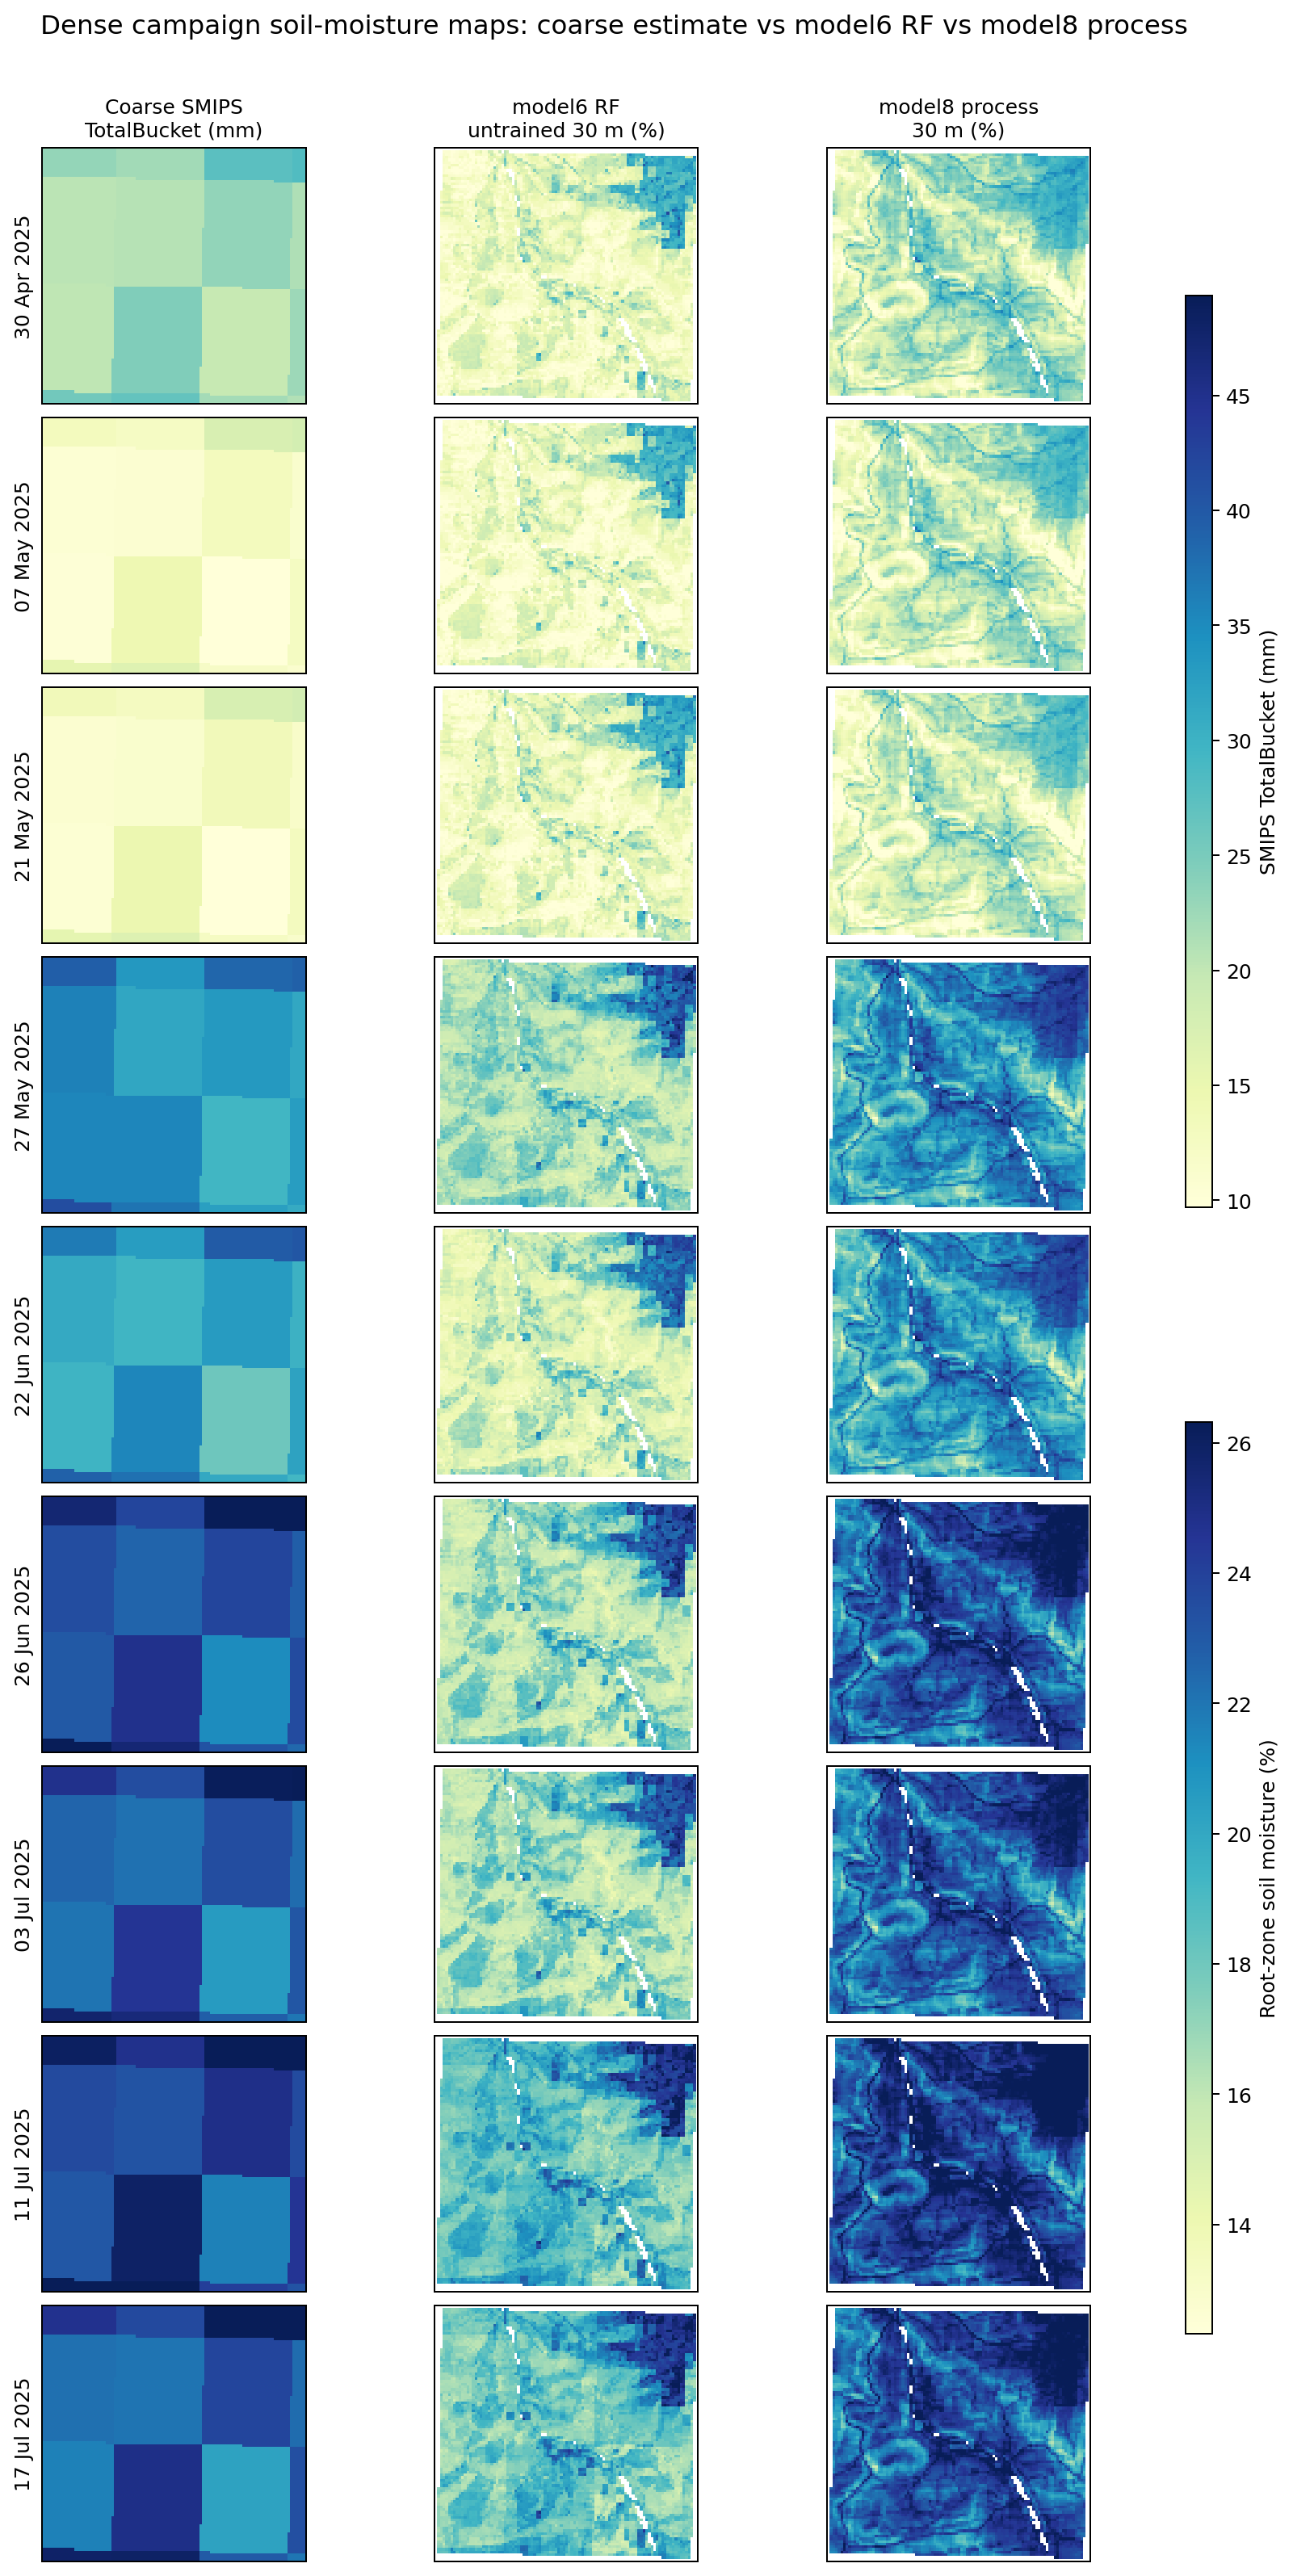
\includegraphics[width=\textwidth]{esdale_coarse_model6_model8_gallery.png}
\caption{Esdale gridded prediction examples: coarse estimate, \modelSix{} and
\modelEight{} for representative dates.  \todo{Verify final selected dry/wet
dates and update caption with observed spatial mean moisture.}}
\label{fig:esdale-gridded}
\end{figure}

\begin{figure}[htbp]
\centering

\includegraphics[width=\textwidth]{tarrawarra_coarse_model6_model8_gallery.png}
\caption{Tarrawarra gridded prediction examples in the 5\,m campaign DEM
footprint.  Validation scores for this site are computed after aggregating raw
TDR observations to model-grid-cell support.  \caution{\modelSix{} also has the
\smips{}-zero caveat for this historical run.}}
\label{fig:tarrawarra-gridded}
\end{figure}

\begin{figure}[htbp]
\centering
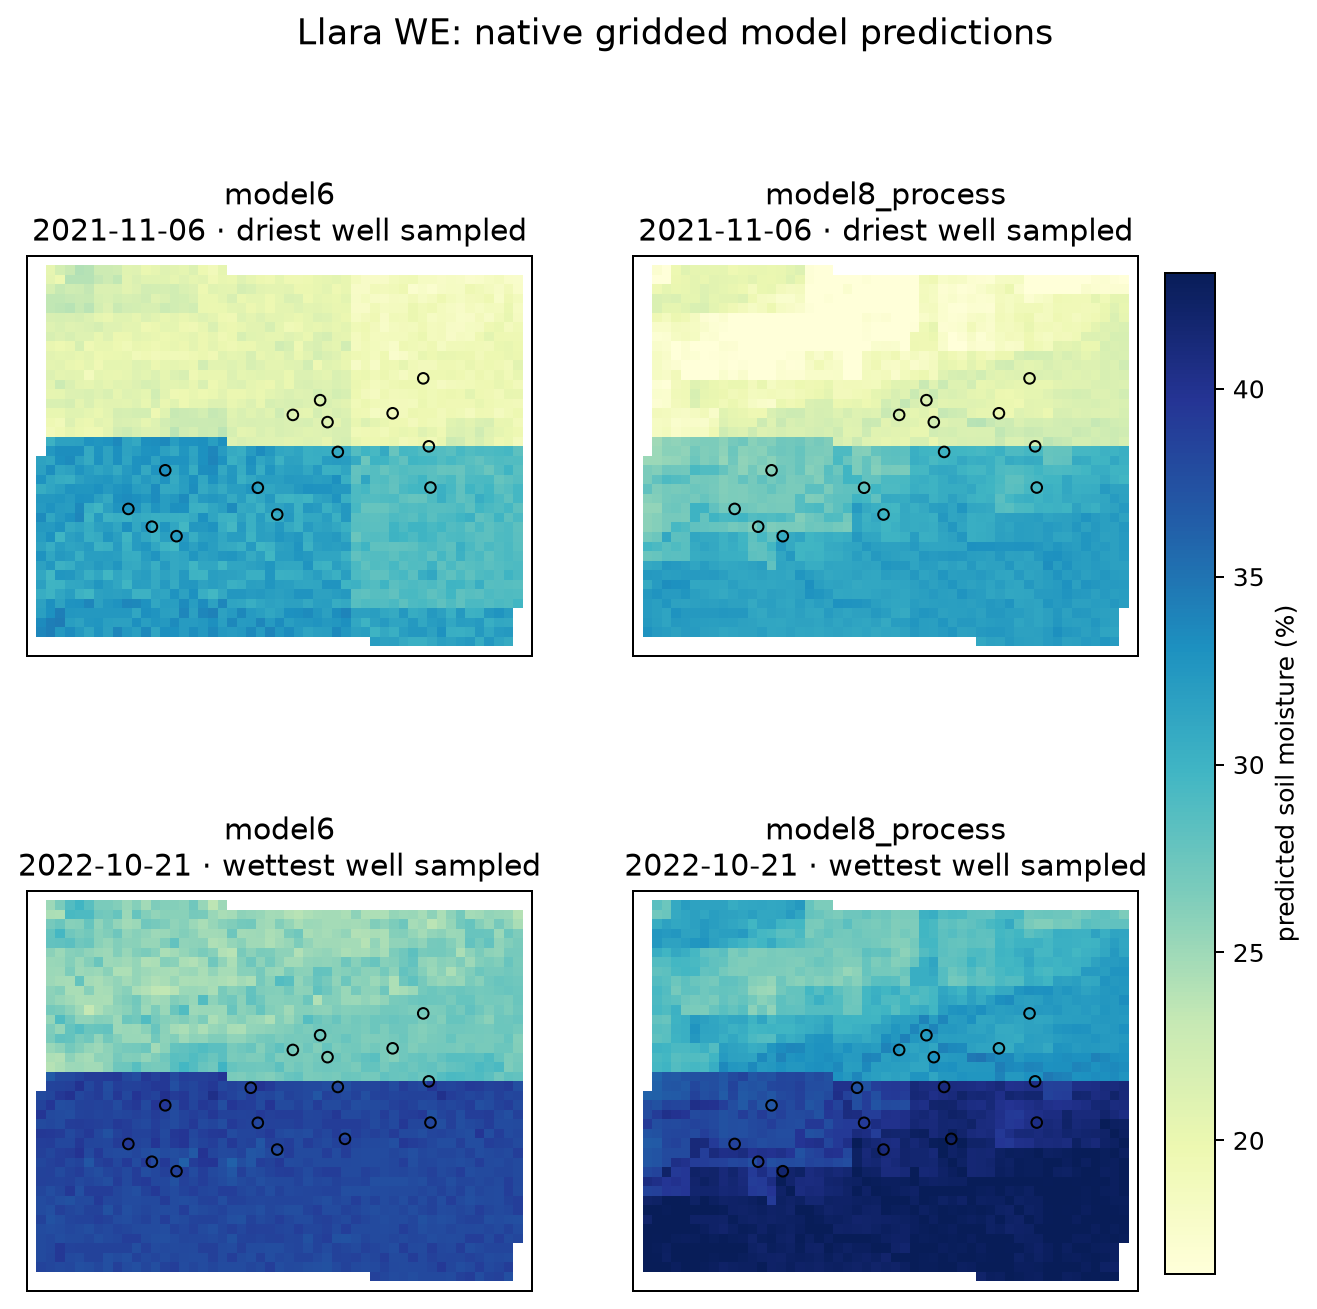
\includegraphics[width=0.49\textwidth]{llara_WE_native_prediction_gallery.png}
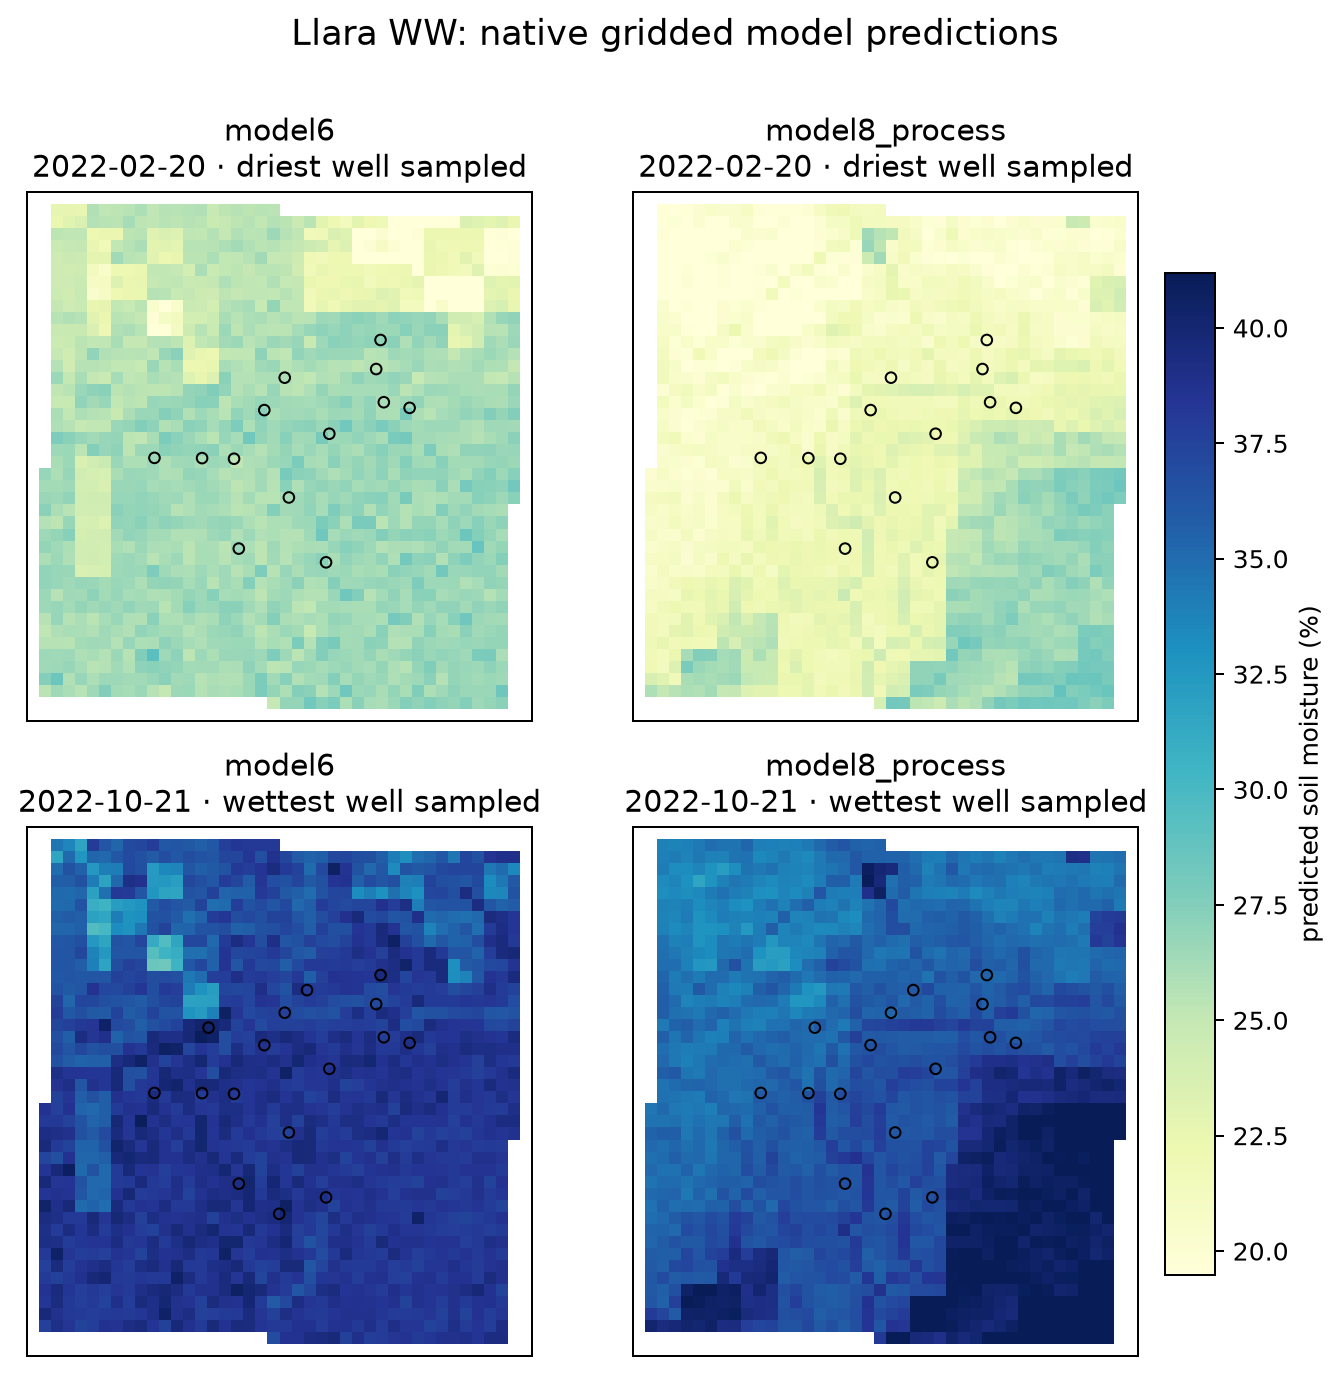
\includegraphics[width=0.49\textwidth]{llara_WW_native_prediction_gallery.png}
\caption{Llara gridded prediction examples for the WE and WW paddocks,
shown separately.  \todo{Consider separate full-width panels in final layout if
the two-paddock figure is too dense.}}
\label{fig:llara-gridded}
\end{figure}

\section{Stage 2: sparse local calibration and local spiking}
\label{sec:stage2}

\subsection{Rationale}\label{sec:stage2-rationale}

Independent validation tells us where the national/global model fails.  A
deployment question follows: can a small amount of local information correct
site-level or terrain-conditioned bias without requiring dense sampling at
every property?  This stage should be interpreted as a local adaptation
experiment, not as independent validation of the base models.

The experiment should mimic realistic local information.  A new landholder
will usually not know where the model performs badly, but may know where the
landscape is generally wet, dry, low, high, clayey or exposed.  Calibration
point selection should therefore compare random selection against simple
landscape-knowledge proxies and model-informed extremes.

\subsection{Calibration layers and point-selection strategies}
\label{sec:stage2-methods}

The current calibration layers are:

\begin{enumerate}
\item \textbf{Bias offset:} one constant residual correction.
\item \textbf{Seasonal offset:} separate residual offsets by season where
  enough dates exist.
\item \textbf{Affine correction:} local linear rescaling of prediction level.
\item \textbf{Residual ridge layer:} residual model using selected model-input
  covariates.
\end{enumerate}

Point budgets are one, three, five, ten, 25\,\%, 50\,\% and all eligible local
calibration points.  Validation is performed on held-out points and dates, with
the strict spatial+temporal block treated as the primary transfer estimate.

\todo{State exactly which selection strategies are retained in the final
protocol.  Candidate final set: random, field-knowledge wet/dry proxy,
global-prediction extremes, terrain-representative.}

\subsection{Learning curves}\label{sec:stage2-learning}

\begin{figure}[htbp]
\centering

\includegraphics[width=\textwidth]{random_spatiotemporal_learning_curves_rmse_gain.png}
\caption{Sparse local-calibration learning curves under strict spatial+temporal
blocking.  Positive values indicate lower RMSE after calibration.  \todo{Update
caption with the minimum point budget needed to achieve material improvement by
site and model.}}
\label{fig:learning-curves}
\end{figure}

\subsection{One-sensor placement strategies}\label{sec:stage2-one-sensor}

\begin{figure}[htbp]
\centering

\includegraphics[width=0.9\textwidth]{one_sensor_strategy_comparison_rmse_gain.png}
\caption{One-sensor selection strategy comparison.  This figure addresses the
deployment question: if only one local point can be instrumented, should it be
chosen randomly, by landscape knowledge, or by model-informed wet/dry
extremes?  \todo{Add final inference by site.}}
\label{fig:one-sensor}
\end{figure}

\subsection{Do process and statistical models respond differently?}
\label{sec:stage2-process-vs-statistical}

The process-vs-statistical comparison is both technical and philosophical.  A
statistical downscaler may already encode nonlinear terrain and soil
relationships learned from the station network, but it may be brittle outside
the training distribution.  A process model may have simpler temporal dynamics
and fewer degrees of freedom, but a local layer may correct its site-level
state more cleanly.  Dense datasets allow this difference to be measured as
the marginal gain from the same sparse local information.

\begin{figure}[htbp]
\centering

\includegraphics[width=0.9\textwidth]{process_vs_statistical_responsiveness_random.png}
\caption{Process-vs-statistical local calibration responsiveness.  Positive
values indicate that \modelEight{} gained more RMSE improvement than
\modelSix{} from the same sparse local information budget.  \todo{Confirm
whether the final figure should use random selection only or the best
realistic selection strategy per site.}}
\label{fig:process-response}
\end{figure}

\section{Discussion}\label{sec:discussion}

\subsection{What dense validation adds beyond station validation}
\label{sec:dense-adds}

\todo{Synthesis paragraph.  Suggested claim: the companion paper establishes
regional/station transfer; dense validation reveals whether the 30\,m product
has meaningful within-site spatial structure and whether residuals organise by
terrain, season and wetness state.}

\subsection{Model complementarity at paddock scale}
\label{sec:model-complementarity}

\todo{Discuss whether \modelSix{} and \modelEight{} fail in the same places.
Use paired comparisons and maps.  Avoid a single global winner unless the
paired evidence is strong and caveats are resolved.}

\subsection{Implications for local deployment}
\label{sec:deployment}

\todo{Discuss the one-sensor / few-sensor deployment story.  Frame local
calibration as a separate adaptation layer placed on top of a national/global
model, not as leakage into independent validation.}

\subsection{Future public training and validation data}
\label{sec:future-data}

\todo{Discuss likely value of additional public dense datasets, sensor
networks, campaign data and remote/proximal sensing products.  Separate data
that improve model training from data that improve independent validation.}

\section{Limitations}\label{sec:limitations}

\begin{itemize}
\item Esdale has strong spatial/terrain coverage but short autumn--winter
coverage.
\item Llara has strong temporal/seasonal coverage but only 32 probes across
two paddocks.
\item Tarrawarra has exceptional raw point density; validation now aggregates
those points to model grid cells by date before scoring. The current
\modelSix{} \smips{}-zero caveat prevents direct interpretation as an
operational \modelSix{} result. High within-cell TDR variance should be treated
as support mismatch unless future models explicitly represent sub-pixel
structure.
\item Soil-moisture depth definitions and profile integration differ across
datasets and must be documented carefully.
\item Dense datasets remain limited in climate and soil coverage relative to
the intended national product.
\item \nse{} can be unstable when observed variance is small; Pearson
$\pearsonr$, RMSE, \ubrmse{} and bias must be interpreted alongside it.
\item Local calibration experiments are deployment sensitivity analyses, not
independent validation of the base models.
\end{itemize}

\section{Conclusions}\label{sec:conclusions}

\todo{Write as 4--6 numbered conclusions.  Suggested structure:
(1) dense validation is a distinct evidence layer; (2) headline independent
skill and caveats; (3) seasonal/wetness/terrain bias; (4) model6/model8
complementarity; (5) sparse local calibration implications; (6) priority next
data.}

\section*{Code and data availability}

All validation code and report-generation scripts are maintained in the
\texttt{DMM\_validation} repository.  Model definitions and the companion paper
are maintained in the \texttt{DownscalingMoistureModel} repository.
\todo{Add repository URLs, branch names, commit hashes, data access statements
and any restrictions before submission.}

\section*{Supplementary material plan}

\begin{itemize}
\item Full model-agnostic prediction tables for Esdale, Tarrawarra and Llara.
\item Full per-site/model metric tables.
\item Full terrain/model-input strata tables.
\item Full paired support/date model comparison tables.
\item Local calibration design tables, selected calibration points and
  replicate-level learning-curve outputs.
\item Additional prediction-quality maps and gridded dry/wet map examples.
\end{itemize}

\bibliographystyle{plainnat}
\bibliography{../../../DownscalingMoistureModel/paper/references,references_dense_validation}

\end{document}
